\documentclass[]{beamer}
% hyperref={pdfpagelabels=false} in [] bei documentclass

\usepackage[utf8]{inputenc}
\usepackage[T1]{fontenc}
\usepackage[ngerman]{babel}
\usepackage{subfigure}
\usepackage{braket}
\usepackage{appendixnumberbeamer}
\usepackage{booktabs}
\usepackage{pgfplots}
\usepackage{xspace}
\usepackage{amsmath, amssymb, amsthm}
%\usepackage{footmisc}

%usepackage[]{footmisc}

\usetheme[numbering=none, progressbar=frametitle]{metropolis}
%\metroset{numbering=none}

\title{Qubits als Bestandteile von Quantencomputern}
\subtitle{Präsentation der Seminarfacharbeit}

\author{Philip Geißler, Joe Schaller, Alexander von Mach}
\date{Jena, 10. Januar 2018}

\usepackage{tikz}
\usetikzlibrary{ipe, arrows.meta}

%\usepackage{mathtools}

\begin{document}

\frame{\titlepage}

%Am Anfang undurchlässig
%Dann durchlässig
\addcontentsline{toc}{section}{Besonderheiten von Polarisationsfiltern}
\begin{frame}{Besonderheiten von Polarisationsfiltern}
	\begin{figure}
	\only<1>{
    \subfigure[$0^\circ$ Winkeldifferenz]{
    	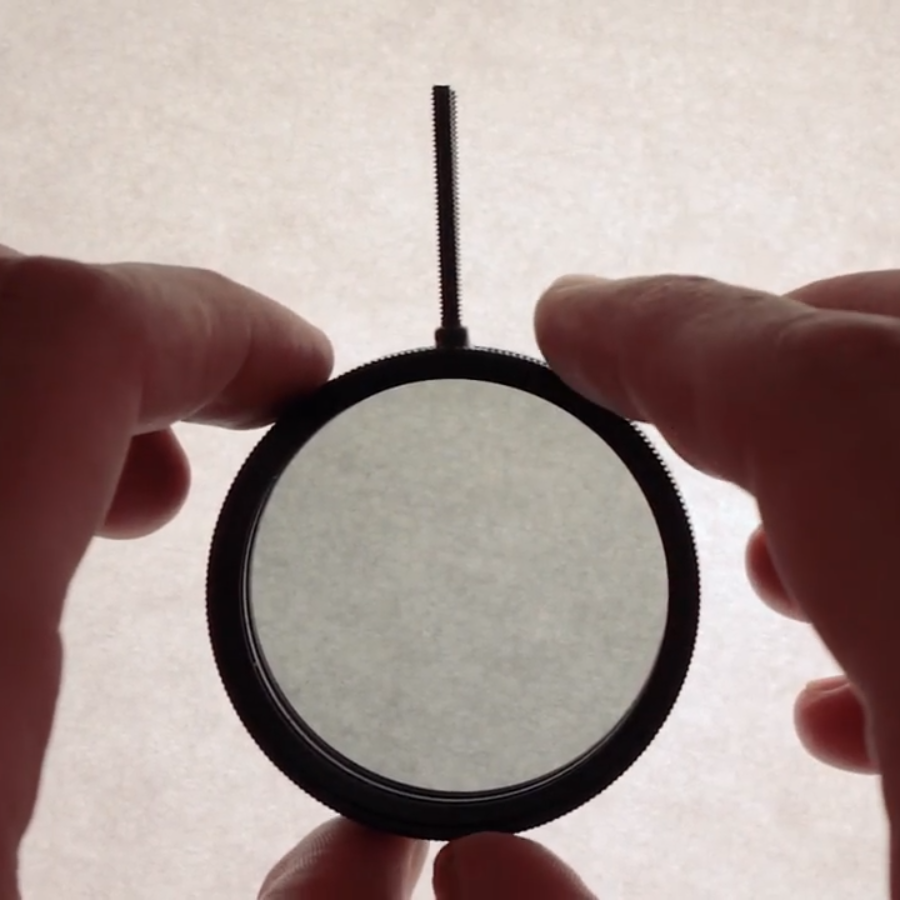
\includegraphics[width=0.47\textwidth]{Parallel.png}
    }
    \subfigure[$90^\circ$ Winkeldifferenz]{
    	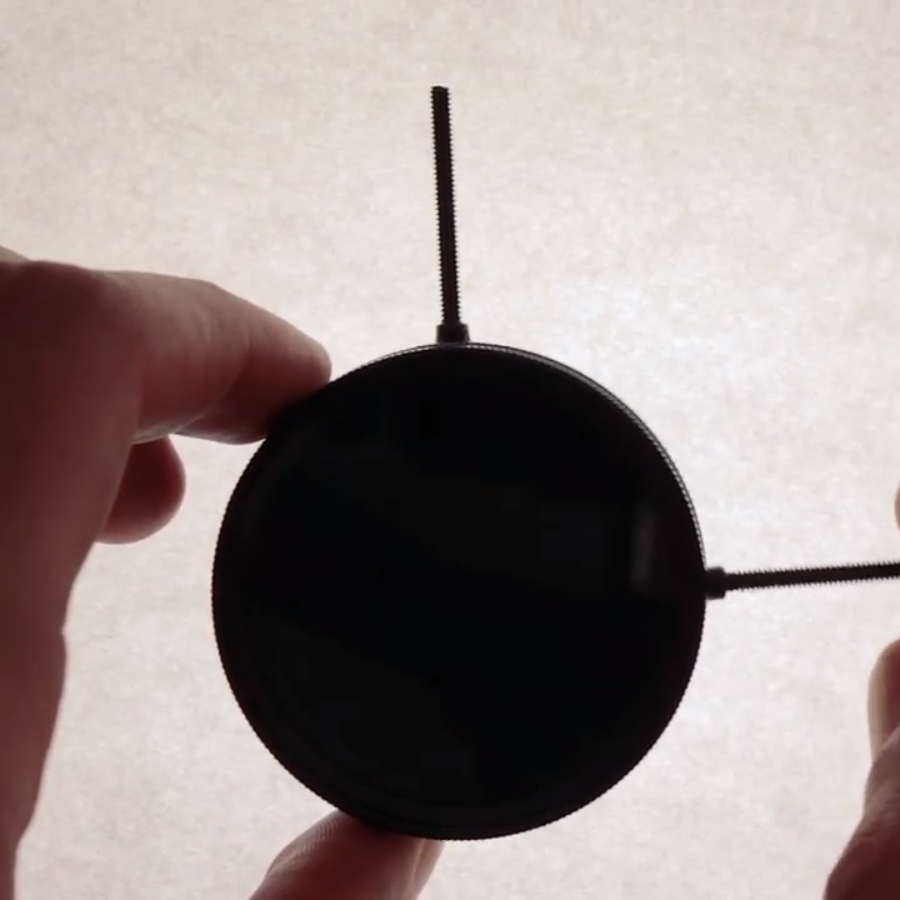
\includegraphics[width=0.47\textwidth]{Orthogonal.png}
    }
    }
    \only<2>{
    \subfigure[Schnittfläche undurchlässig]{
    	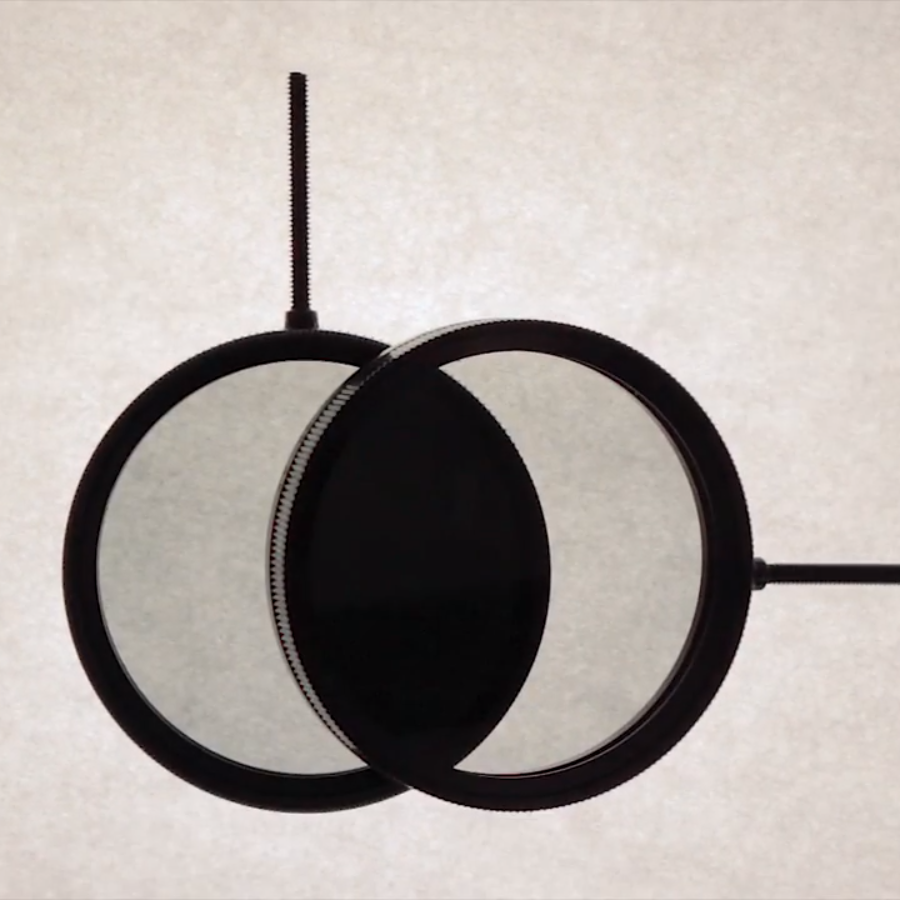
\includegraphics[width=0.47\textwidth]{Ortho2Venn.png}
    }
    \subfigure[mit Zusatz wieder durchlässig]{
    	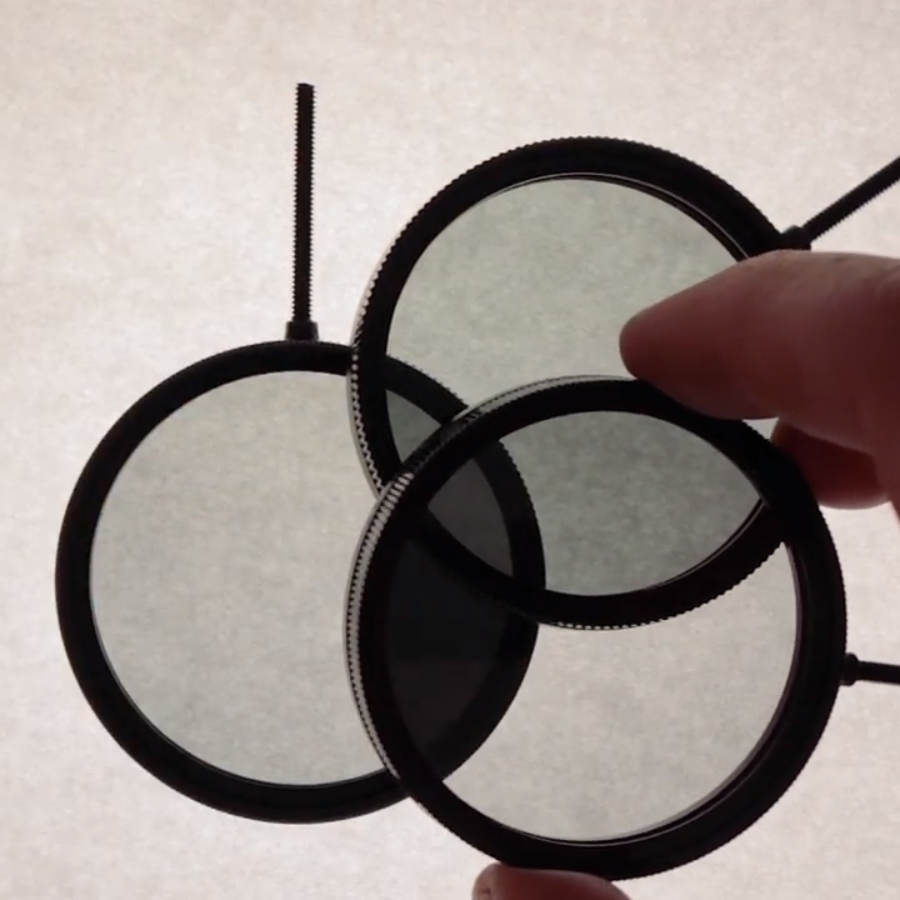
\includegraphics[width=0.47\textwidth]{3Venn.png}
    }
    }
	\caption{Verhalten von Polarisationsfiltern\footnote{Henry Reich, September 2017, 1:00 - 2:00}}
	\end{figure}
\end{frame}

%\addcontentsline{toc}{section}{Table of Contents}
\begin{frame}{Gliederung}
%\setbeamertemplate{section in toc}[sections numbered]
\tableofcontents
\end{frame}

\section{Qubits und Quantencomputer}
\subsection{Allgemeine Grundlagen}
\begin{frame}{Allgemeine Grundlagen: Computer vs. Quantencomputer}
\begin{center}
	\begin{itemize}
	\item Computer arbeitet mit Bits
    \item Zustände 0 und 1
    \item Daten in Reihen von 8 Bits aufgeteilt
    \item Logische Gatter zur Zustandsänderung
	\end{itemize}
\end{center}
\end{frame}

\begin{frame}{Allgemeine Grundlagen: Computer vs. Quantencomputer}
\begin{center}
	\begin{itemize}
	\item Quantencomputer arbeitet mit Qubits
    \item Zustände 0 und 1
    \item Reihen von Zuständen bilden Daten
    \item Quantengatter zur Zustandsänderung
    \item Superpositions- und Verschränkungszustände
	\end{itemize}
\end{center}
\end{frame}

\begin{frame}{Allgemeine Grundlagen: Superpositionen}
\begin{center}
\begin{figure}
  		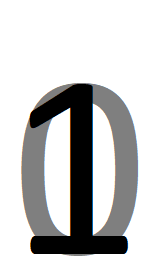
\includegraphics[width=0.15\linewidth]{Bild2.png}
 	 	\caption{Superposition}
 	 	\centering
  	\end{figure}
	\begin{itemize}
	\item Quantencomputer arbeitet mit Wahrscheinlichkeiten
    \item Bei Messung zerfällt die Superposition
    \item Zustand dann entweder 0 oder 1
	\end{itemize}
\end{center}
\end{frame}

\begin{frame}{Allgemeine Grundlagen: Schrödingers Katze}
\begin{center}
\begin{figure}
  		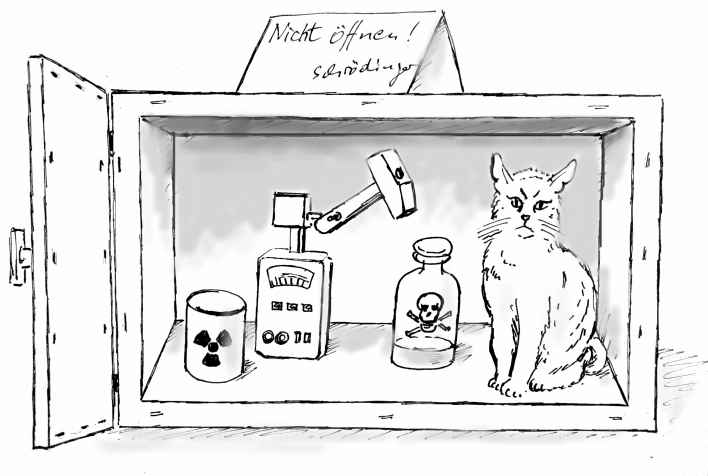
\includegraphics[width=0.5\linewidth]{katze.jpg}
 	 	\caption{Schrödingers Katze ~ \footnotesize{\url{http://bit.ly/2CUIBoZ}, 4.1.2018}}
 	 	\centering
  	\end{figure}
	\begin{itemize}
    \item Katze in Box mit radioaktiver Probe
	\item Box geschlossen: Katze tot und lebendig
    \item Öffnen der Box: Superposition zerfällt
	\end{itemize}
\end{center}
\end{frame}

\begin{frame}{Allgemeine Grundlagen: Physikalische Qubitrepräsentation}
\begin{center}
\begin{itemize}
 \item Qubits können in verschiedener Form erschaffen werden
 \item Teilchen wird zum Qubit durch Energiezufuhr
 \item Qubit aus Grundzustand in eine Superposition gebracht
\end{itemize}

\end{center}
\end{frame}

\begin{frame}{Allgemeine Grundlagen: Physikalische Qubitrepräsentation}
\begin{center}
\begin{itemize}
  \item Wird das Qubit observiert gibt es seinen Zustand Preis
  \item dann kann es angeregt oder nicht angeregt sein
  \end{itemize}
  	\begin{figure}
  		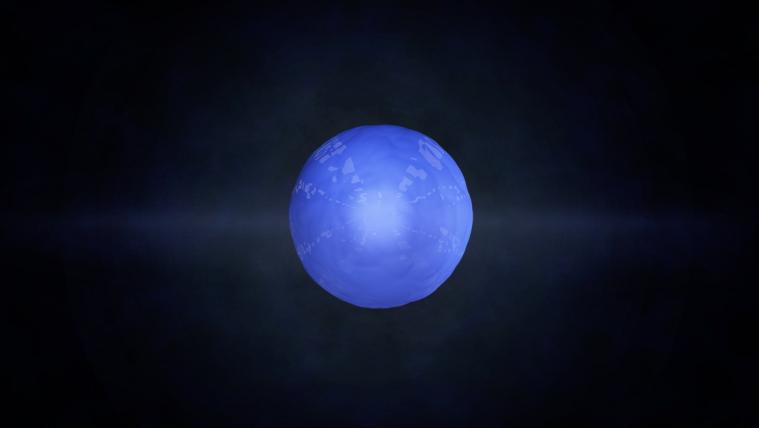
\includegraphics[width=0.6\linewidth]{Bild_1.jpg}
 	 	\caption{Quant \newline \footnotesize{\url{https://app.curiositystream.com/video/737/properties-of-a-qubit},04.01.2018}}
 	 	\centering
  	\end{figure}
\end{center}
\end{frame}


\begin{frame}{Allgemeine Grundlagen: Technische Qubitumsetzungen}
\begin{center}
\begin{itemize}
	\item in Realität gibt es bisher keinen Quantencomputer
    \item verschiedene Arten haben verschiedene Umsetzungsmöglichkeiten %einbringender Vergleich zu Regulären computern Zum peispiel
    \item vielversprechendste Form: die Ionenfalle
    \item Anregung von Ionen durch elektromagnetische Impulse
    \item Erschaffen von bis zu 16 verschränkten Qubits %anbringen der Tatsacke einer 2^32 stelligen matrix
\end{itemize}
\end{center}
\end{frame}

\begin{frame}{Allgemeine Grundlagen: Technische Qubitumsetzungen}
\begin{center}
	\begin{itemize}
	\item Größte Probleme sind die schweren Bedingungen
    \item Qubits müssen auf wenige Millikelvin heruntergekühlt sein
    \item Qubits im Grundzustand müssen völlig abgeschirmt sein
    \item Zeitintervalle im Superpositionszustand sind sehr kurz
    \item in realen Quantencomputern können zufällige Fehler auftreten
\end{itemize}
\end{center}
\end{frame}

\begin{frame}{Allgemeine Grundlagen: Technische Qubitumsetzungen}
\begin{center}
	\begin{figure}
  		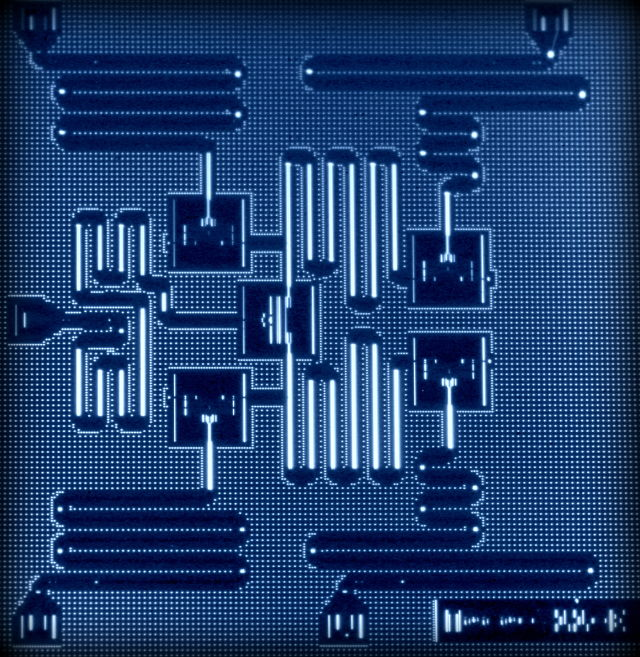
\includegraphics[width=0.5\linewidth]{Bild3.jpg}
 	 	\caption{ibmqx2 \newline\footnotesize{\url{https://arstechnica.com/science/2016/05/how-ibms-new-five-qubit-universal-quantum-computer-works/}, 02.01.2018}}
 	 	\centering
  	\end{figure}
\end{center}
\end{frame}


\begin{frame}{Allgemeine Grundlagen: Grundzustände von Qubits}
\begin{center}
	\begin{itemize}
	\item 2 Qubits erzeugen 4 Grundzustände
    \item $\ket{00}$,$\ket{01}$, $\ket{10}$,$\ket{11}$
    \item 3 Qubits erzeugen 8 Grundzustände
    \item n Qubits erzeugen damit $2^n$ Grundzustände
	\end{itemize}
\end{center}
\end{frame}


\begin{frame}{Allgemeine Grundlagen: Mathematische Darstellung einer Superposition}
\begin{center}
	\begin{itemize}
	\item $\sqrt[]{\alpha} \cdot  \ket{0} + \sqrt[]{\beta} \cdot \ket{1}$ mit $\sqrt{|\alpha|^2 + |\beta|^2} = 1$
	\item $\ket{00}$ + Gatter =  $\sqrt[]{1/2} \cdot  \ket{01} + \sqrt[]{1/2} \cdot \ket{10}$
    \item Superposition abhängig von angewendetem Gatter
    \item Wert im Wurzelterm gibt an bei wie vielen Messungen ein bestimmter Zustand eintritt
	\end{itemize}
\end{center}
\end{frame}

\begin{frame}{Allgemeine Grundlagen: Quantengatter und deren Verhaltensweisen}
\begin{center} %Alex
	\begin{itemize}
	\item Quantengatter verändern Superpositionszustand eines Qubits
    \item Zustände und Wahrscheinlichkeiten ändern sich
    \item so können durch Messung statistische Ergebnisse erzielt werden
\end{itemize}
\end{center}
\end{frame}

\begin{frame}{Allgemeine Grundlagen: Observieren von Quantengattern}
\begin{center} %Alex
	\begin{itemize}
	\item ein Qubit in einer Superposition kann nach Messung nur 0 oder 1 ausgeben so wie ein klassischer Computer
    \item mehrere Qubits können viele verschiedene Kombinationen aus 0 und 1 ausgeben
    \item so können mehrere Ergebnisse gleichzeitig erzeugt werden
\end{itemize}
\end{center}
\end{frame}

\subsection{Mathematische Verhaltensweise eines Qubits}
\begin{frame}{Mathematische Verhaltensweise: Vektordarstellung eines Qubits}%Alex
\begin{center}
	\begin{itemize}
 \item Darstellung der Superposition eines Qubits am Einheitskreis
 \item Länge des resultierenden Vektors aus den einzelnen Komponenten ist immer 1
 \item $\sqrt{\vert a \vert^2 +\vert b\vert^2}$
 \item unabhängig von der Dimension
\end{itemize}
\end{center}
\end{frame}

\begin{frame}{Mathematische Verhaltensweise: Komplexe Zahlen}%Alex
\begin{center}
\begin{itemize}
	\item Komplexe Zahlen sind eine weiter Dimension am Zahlenstrahl
    \item eine Einheit i im Komplexen Bereich kann dargestellt werden als $\sqrt{-1}$
    \item $i^2 = -1$
\end{itemize}
\end{center}
\end{frame}

\begin{frame}{Mathematische Verhaltensweise: Amplituden der Wahrscheinlichkeiten}%Alex
\begin{center}
	\begin{itemize}
	\item da $\sqrt{\vert a\vert^2 + \vert b\vert^2} = 1$ müssen die Faktoren wurzeln sein
    \item auch negativen Faktoren da nur Betrag zählt
    \item Beispiel: $\sqrt{1/3} \ket{0110} + \sqrt{1/2} \ket{1010} + \sqrt{1/6} \ket{0000}$
\end{itemize}
\end{center}
\end{frame}

\begin{frame}{Mathematische Verhaltensweise: Demonstration am Einheitskreis}%Alex
\begin{center}
	\begin{itemize}
	 \item Wurzelausdrücke bestimmen die Zustandswahrscheinlichkeit
     \item Der $\ket{}$ Ausdruck beschreibt Zustand, welcher angenommen wird
     \item Die Summe der Betragsquadrate der einzelnen Faktoren ergeben immer 1 %den Rest erklär ich so
\end{itemize}
\begin{figure}
  		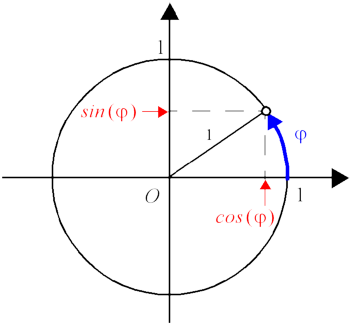
\includegraphics[width=0.35\linewidth]{Bild4.png}
 	 	\caption{Einheitskreis \newline\footnotesize{\url{goo.gl/zuK2aj}, 05.01.2018}}
 	 	\centering
  	\end{figure}
\end{center}
\end{frame}

 \begin{frame}{Mathematische Verhaltensweise: Gatter in der Vektordarstellung}
\begin{center}
	\begin{itemize}
	\item Gatter bewegen/verändern den Zustandsvektor innerhalb der Einheitskugel
    \item Operationen durch Einheitsmatrix repräsentiert
    \item Multiplikation des Zustandsvektors und der Gattermatrix ergibt neuen Zustand
	\end{itemize}
\end{center}
\end{frame}

\begin{frame}{Mathematische Verhaltensweise: Matrizen und Bewegungen ausgewählter Gatter}
\begin{center}%xyzh
	\begin{itemize}
	\item Hadamard-Gatter \begin{itemize}
    \item erzeugt Superpositionszustand
	\item Gerade Anzahl -> Anfangszustand
	\end{itemize}
	\end{itemize}
    \begin{align*}
H= 1/\sqrt{2} \begin{bmatrix} 1&1\\1&-1\\\end{bmatrix} &
\end{align*}
\end{center}
\end{frame}

\begin{frame}{Mathematische Verhaltensweise: Matrizen und Bewegungen ausgewählter Gatter}
\begin{center}%xyzh
	\begin{itemize}
	\item Pauli-Gatter \begin{itemize}
    \item einfache Qubitoperationen
    \item X-, Y-, Z- Pauli-Gatter
    \item X-Pauli-Gatter negiert die Amplituden der Grundzustände
	\end{itemize}
	\end{itemize}
    \begin{align*}X= \begin{bmatrix} 0&1\\1&0\\\end{bmatrix} &\end{align*} \\
\end{center}
\end{frame}

\begin{frame}{Mathematische Verhaltensweise: Matrizen und Bewegungen ausgewählter Gatter}
\begin{center}
\begin{itemize}
\item Negation der Phasen von X und Z
\item Amplitude der Grundzustände wird vertauscht
\item Kombination aus X und Z
\end{itemize}
\begin{align*}Y= \begin{bmatrix} 0&-i\\i&0\\\end{bmatrix} &\end{align*}
\end{center}
\end{frame}

\begin{frame}{Mathematische Verhaltensweise: Matrizen und Bewegungen ausgewählter Gatter}
\begin{center}
\begin{itemize}
\item Spiegelung des Zustandes an der Z-Achse
\item Messung immer in Z-Richtung, daher keine Änderung des Ergebnisses
\end{itemize}
\begin{align*}Z= \begin{bmatrix} 1&0\\0&-1\\\end{bmatrix} &\end{align*}
\end{center}
\end{frame}

\subsection{Möglichkeiten des Quantencomputers}

\begin{frame}{Möglichkeiten des Quantencomputers: Parallelisieren von Rechnungen}
\begin{center}
	\begin{itemize}
	\item durch Superposition ermöglicht
	\item Beispiel: 6-Qubit-System
    \item Quantencomputer operiert auf Ebenen des Lösungsbaums \footnote{Houston-Edwards, 2017}
    \item mehrere Durchläufe bis zur Korrekten Lösung

	\end{itemize}
\end{center}
\end{frame}

\begin{frame}{Möglichkeiten des Quantencomputers: Algorithmus von Shor}
\begin{center}
	\begin{itemize}
	\item 1994 von Peter Shor veröffentlicht
    \item speziell für Quantencomputer entworfen
    \item dient der Berechnung nichttrivialer Teiler von Zahlen und ist damit ein Faktorisierungsverfahren\footnote{Paul, Zoppke, 2002}
    \item bisher nur einige experimentelle Versuche

	\end{itemize}
\end{center}
\end{frame}

\section{Belltheorem und Quantencomputersimulation}

\begin{frame}{Kontroversen der Quantenphysik}
\begin{center}
	\begin{huge}
	\textit{\glqq Gott würfelt nicht!\grqq{}\hspace{1mm}\footnote{Albert Einstein, 4. Dezember 1926}}
	\end{huge}
\end{center}
\end{frame}

\begin{frame}{Kontroversen der Quantenphysik}
\only<2>{\begin{table}
    \only<2>{\begin{tabular}{l|l}
      \toprule
      Lokalität \& Realismus \hspace{1.6cm} & Verschränkung \& Superposition\\
      \midrule
      $\Rightarrow$ Erklärbarkeit der Phänomene & $\Rightarrow$ Ablehnung des lokalen \\
      \qquad durch \glqq versteckte\grqq{} Variablen & \qquad Realismus'\\
      $\Rightarrow$ Berechenbarkeit der & $\Rightarrow$ Unberechenbarkeit der\\
      \qquad \textbf{Ergebnisse} im Voraus & \qquad \textbf{Ergebnisse}\\
      \qquad (mit genügend Daten) & \qquad im Voraus\\
      %\bottomrule
    \end{tabular}}
    \vspace{0.5cm}
    \caption{Interpretationen der Quantenphysik während ihrer Anfänge}
  \end{table}
}
\only<1>{
\textbf{Lokalität:}
\glqq Interaktionen und Informationsübertragungen können höchstens mit Lichtgeschwindigkeit stattfinden.\grqq$^5$

\textbf{Realismus:}
\glqq Messgrößen werden durch Objekteigenschaften bestimmt, die unmit­telbar vor der Messung tatsächlich vorliegen.\grqq\footnote{Dr. Gebhard Greiter, Dezember 2017, S.1}


\textbf{Verschränkung:}
\glqq Unbeschreibbarkeit eines $n$-Qubit Systems durch die Beschreibung der einzelnen Teilsysteme.\grqq$^6$

\textbf{Superposition:}
\glqq Die Eigenschaft der Möglichkeit des Existierens eines Qubits in mehreren Qubitzuständen.\grqq\footnote{Colm Heigeartaigh, Mai 2005, S.2}
}
\end{frame}

\begin{frame}{Kontroversen der Quantenphysik}
\begin{center}
	\begin{large}
	Gibt es ein Experiment, für das die beiden Ansätze ein unterschiedliches Ergebnis vorhersagen?\\~\\~\\
	\end{large}

	\alert{
	\begin{huge}
	~~~~
	\end{huge}
	}
\end{center}
\end{frame}

\begin{frame}{Kontroversen der Quantenphysik}
\begin{center}
	\begin{large}
	Gibt es ein Experiment, für das die beiden Ansätze ein unterschiedliches Ergebnis vorhersagen?\\~\\~\\
	\end{large}

	\alert{
	\begin{huge}
	Belltest
	\end{huge}
	}
\end{center}
\end{frame}

\begin{frame}{Belltest}
\begin{center}
Annahme: Jedes Photon besitzt versteckte Variablen, die eindeutig festlegen, durch welche Polarisationsfilter dieses geblockt wird.
\end{center}
\vspace{-0.5cm}
\begin{align*}
 	1 &= p(a)&
 	1&\geqslant p(b)&
 	1&\geqslant p(c)
\end{align*}
\vspace{-1cm}
\begin{align*}
 	p(b)+p(\neg b) &\geqslant p(b)\\
 	p(a)\cdot p(b) \cdot p(c) + p(a)\cdot p(\neg b) \cdot p(c) &\geqslant p(a)\cdot p(b) \cdot p(c)\\
 	p(a \wedge b \wedge c)+p(a \wedge \neg b \wedge c) &\geqslant p(a \wedge b \wedge c)\\
 	p(a \wedge c) &\geqslant p(a \wedge b \wedge c)
\end{align*}
\end{frame}

\begin{frame}{Belltest}
\begin{center}
 Annahme: Jedes Photon besitzt versteckte Variablen, die eindeutig festlegen, durch welche Polarisationsfilter dieses geblockt wird.
\end{center}
\vspace{-0.5cm}
\begin{align*}
 	1 &= p(a)&
 	1&\geqslant p(b)&
 	1&\geqslant p(c)
\end{align*}
\vspace{-1cm}
\begin{align*}
 	p(b)+p(\neg b) &\geqslant p(b)\\
 	p(a)\cdot p(b) \cdot p(c) + p(a)\cdot p(\neg b) \cdot p(c) &\geqslant p(a)\cdot p(b) \cdot p(c)\\
 	p(a \wedge b \wedge c)+p(a \wedge \neg b \wedge c) &\geqslant p(a \wedge b \wedge c)\\
 	p(a \wedge c) &\geqslant p(a \wedge b \wedge c)\\
 	0\% &\geqslant x &| x>0\%\\
 	Wider&spruch
\end{align*}
\end{frame}

\begin{frame}{Belltest}
\begin{figure}
	%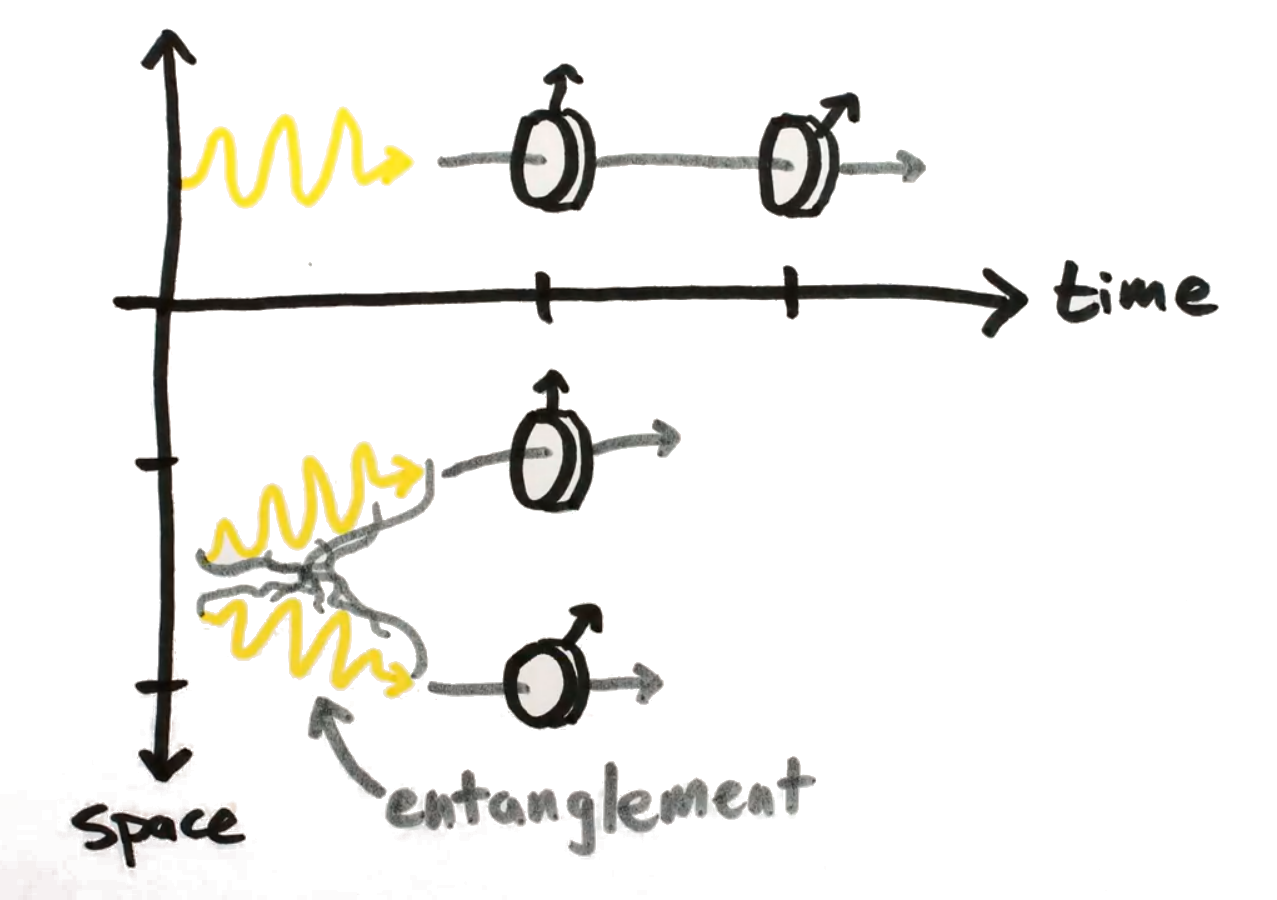
\includegraphics[width=0.35\linewidth]{bell2.png}
	\definecolor{red}{rgb}{1,0,0}
\definecolor{green}{rgb}{0,1,0}
\definecolor{blue}{rgb}{0,0,1}
\definecolor{yellow}{rgb}{1,1,0}
\definecolor{orange}{rgb}{1,0.5,0}
\definecolor{purple}{rgb}{0.75,0,0.25}
\definecolor{gray}{rgb}{0.5,0.5,0.5}
\definecolor{brown}{rgb}{0.75,0.5,0.25}
\definecolor{pink}{rgb}{1,0.75,0.75}
\definecolor{violet}{rgb}{0.5,0,0.5}
\definecolor{darkgray}{rgb}{0.25,0.25,0.25}
\definecolor{lightgray}{rgb}{0.75,0.75,0.75}
\definecolor{lime}{rgb}{0.75,1,0}
\definecolor{teal}{rgb}{0,0.5,0.5}
\definecolor{cyan}{rgb}{0,1,1}
\definecolor{magenta}{rgb}{1,0,1}
\definecolor{olive}{rgb}{0.5,0.5,0}
\definecolor{gold}{rgb}{1,0.843,0}
\definecolor{navy}{rgb}{0,0,0.502}
\definecolor{seagreen}{rgb}{0.18,0.545,0.341}
\definecolor{turquoise}{rgb}{0.251,0.878,0.816}
\definecolor{darkblue}{rgb}{0,0,0.545}
\definecolor{darkcyan}{rgb}{0,0.545,0.545}
\definecolor{darkgreen}{rgb}{0,0.392,0}
\definecolor{darkmagenta}{rgb}{0.545,0,0.545}
\definecolor{darkorange}{rgb}{1,0.549,0}
\definecolor{darkred}{rgb}{0.545,0,0}
\definecolor{lightblue}{rgb}{0.678,0.847,0.902}
\definecolor{lightcyan}{rgb}{0.878,1,1}
\definecolor{lightgreen}{rgb}{0.565,0.933,0.565}
\definecolor{lightyellow}{rgb}{1,1,0.878}
\definecolor{black}{rgb}{0,0,0}
\definecolor{white}{rgb}{1,1,1}
\begin{tikzpicture}[ipe import, scale=0.6, every node/.style={transform shape}]
  \draw[shift={(144, 280)}, yscale=0.7619, very thick, ->]
    (0, 0)
     -- (0, 336);
  \draw[shift={(128, 368)}, xscale=0.9167, very thick, ->]
    (0, 0)
     -- (384, 0);
  \filldraw[shift={(280, 296)}, scale=0.5, thick, fill=darkgray]
    (0, 0)
     arc[start angle=89.9999, end angle=269.9999, x radius=-16, y radius=-56]
     -- (-16, 112)
     { [rotate=0.0001] arc[start angle=89.9996, end angle=269.9996, x radius=16, y radius=56] }
     -- cycle;
  \filldraw[thick, fill=darkorange]
    (272, 324) ellipse[x radius=8, y radius=28];
  \draw[shift={(272, 308)}, scale=0.5, thick, ->]
    (0, 0)
     -- (0, 64);
  \filldraw[shift={(380, 384)}, scale=0.5, thick, fill=darkgray]
    (0, 0)
     arc[start angle=89.9999, end angle=269.9999, x radius=-16, y radius=-56]
     -- (-16, 112)
     { [rotate=0.0001] arc[start angle=89.9996, end angle=269.9996, x radius=16, y radius=56] }
     -- cycle;
  \filldraw[thick, fill=darkorange]
    (372, 412) ellipse[x radius=8, y radius=28];
  \draw[shift={(372, 396)}, scale=0.5, thick, ->]
    (0, 0)
     -- (0, 64);
  \filldraw[shift={(380, 296)}, scale=0.5, thick, fill=darkgray]
    (0, 0)
     arc[start angle=89.9999, end angle=269.9999, x radius=-16, y radius=-56]
     -- (-16, 112)
     { [rotate=0.0001] arc[start angle=89.9996, end angle=269.9996, x radius=16, y radius=56] }
     -- cycle;
  \filldraw[thick, fill=darkorange]
    (372, 324) ellipse[x radius=8, y radius=28];
  \draw[thick, ->]
    (368, 324)
     -- (376, 324)
     -- (368, 324)
     -- (376, 324);
  \filldraw[shift={(380, 456)}, scale=0.5, thick, fill=darkgray]
    (0, 0)
     arc[start angle=89.9999, end angle=269.9999, x radius=-16, y radius=-56]
     -- (-16, 112)
     { [rotate=0.0001] arc[start angle=89.9996, end angle=269.9996, x radius=16, y radius=56] }
     -- cycle;
  \filldraw[thick, fill=darkorange]
    (372, 484) ellipse[x radius=8, y radius=28];
  \draw[thick, ->]
    (368, 484)
     -- (376, 484)
     -- (368, 484)
     -- (376, 484);
  \draw[shift={(300, 484)}, xscale=0.8824, semithick, ->]
    (0, 0)
     -- (68, 0);
  \draw[shift={(300, 412)}, xscale=0.8824, semithick, ->]
    (0, 0)
     -- (68, 0);
  \draw[semithick, ->]
    (392, 484)
     -- (432, 484);
  \draw[semithick, ->]
    (392, 412)
     -- (432, 412);
  \draw[shift={(212, 324)}, xscale=0.8571, semithick, ->]
    (0, 0)
     -- (56, 0);
  \draw[semithick, ->]
    (292, 324)
     -- (360, 324);
  \draw[semithick, ->]
    (392, 324)
     -- (432, 324);
  \node[ipe node, font=\large]
     at (152, 528) {Raum};
  \node[ipe node, font=\Huge]
     at (152, 508) {X};
  \node[ipe node, font=\Huge]
     at (464, 372) {T};
  \node[ipe node, font=\LARGE]
     at (432, 372) {Zeit};
  \draw[shift={(256, 484)}, xscale=0.5, gold, very thick]
    (0, 0)
     .. controls (4, 0) and (8, 4) .. (11.3333, 2)
     .. controls (14.6667, 0) and (17.3333, -8) .. (20, -5.3333)
     .. controls (22.6667, -2.6667) and (25.3333, 10.6667) .. (28, 8)
     .. controls (30.6667, 5.3333) and (33.3333, -13.3333) .. (36, -12)
     .. controls (38.6667, -10.6667) and (41.3333, 10.6667) .. (44, 12)
     .. controls (46.6667, 13.3333) and (49.3333, -5.3333) .. (52, -8)
     .. controls (54.6667, -10.6667) and (57.3333, 2.6667) .. (60, 5.3333)
     .. controls (62.6667, 8) and (65.3333, 0) .. (68.6667, -2)
     .. controls (72, -4) and (76, 0) .. (80, 0);
  \draw[shift={(256, 484)}, xscale=0.5, darkorange, thick]
    (0, 0)
     .. controls (4, 0) and (8, 4) .. (11.3333, 2)
     .. controls (14.6667, 0) and (17.3333, -8) .. (20, -5.3333)
     .. controls (22.6667, -2.6667) and (25.3333, 10.6667) .. (28, 8)
     .. controls (30.6667, 5.3333) and (33.3333, -13.3333) .. (36, -12)
     .. controls (38.6667, -10.6667) and (41.3333, 10.6667) .. (44, 12)
     .. controls (46.6667, 13.3333) and (49.3333, -5.3333) .. (52, -8)
     .. controls (54.6667, -10.6667) and (57.3333, 2.6667) .. (60, 5.3333)
     .. controls (62.6667, 8) and (65.3333, 0) .. (68.6667, -2)
     .. controls (72, -4) and (76, 0) .. (80, 0);
  \draw[shift={(168, 484)}, xscale=0.5, gold, very thick]
    (0, 0)
     .. controls (4, 0) and (8, 4) .. (11.3333, 2)
     .. controls (14.6667, 0) and (17.3333, -8) .. (20, -5.3333)
     .. controls (22.6667, -2.6667) and (25.3333, 10.6667) .. (28, 8)
     .. controls (30.6667, 5.3333) and (33.3333, -13.3333) .. (36, -12)
     .. controls (38.6667, -10.6667) and (41.3333, 10.6667) .. (44, 12)
     .. controls (46.6667, 13.3333) and (49.3333, -5.3333) .. (52, -8)
     .. controls (54.6667, -10.6667) and (57.3333, 2.6667) .. (60, 5.3333)
     .. controls (62.6667, 8) and (65.3333, 0) .. (68.6667, -2)
     .. controls (72, -4) and (76, 0) .. (80, 0);
  \draw[shift={(168, 484)}, xscale=0.5, darkorange, thick]
    (0, 0)
     .. controls (4, 0) and (8, 4) .. (11.3333, 2)
     .. controls (14.6667, 0) and (17.3333, -8) .. (20, -5.3333)
     .. controls (22.6667, -2.6667) and (25.3333, 10.6667) .. (28, 8)
     .. controls (30.6667, 5.3333) and (33.3333, -13.3333) .. (36, -12)
     .. controls (38.6667, -10.6667) and (41.3333, 10.6667) .. (44, 12)
     .. controls (46.6667, 13.3333) and (49.3333, -5.3333) .. (52, -8)
     .. controls (54.6667, -10.6667) and (57.3333, 2.6667) .. (60, 5.3333)
     .. controls (62.6667, 8) and (65.3333, 0) .. (68.6667, -2)
     .. controls (72, -4) and (76, 0) .. (80, 0);
  \draw[shift={(168, 412)}, xscale=0.5, gold, very thick]
    (0, 0)
     .. controls (4, 0) and (8, 4) .. (11.3333, 2)
     .. controls (14.6667, 0) and (17.3333, -8) .. (20, -5.3333)
     .. controls (22.6667, -2.6667) and (25.3333, 10.6667) .. (28, 8)
     .. controls (30.6667, 5.3333) and (33.3333, -13.3333) .. (36, -12)
     .. controls (38.6667, -10.6667) and (41.3333, 10.6667) .. (44, 12)
     .. controls (46.6667, 13.3333) and (49.3333, -5.3333) .. (52, -8)
     .. controls (54.6667, -10.6667) and (57.3333, 2.6667) .. (60, 5.3333)
     .. controls (62.6667, 8) and (65.3333, 0) .. (68.6667, -2)
     .. controls (72, -4) and (76, 0) .. (80, 0);
  \draw[shift={(168, 412)}, xscale=0.5, darkorange, thick]
    (0, 0)
     .. controls (4, 0) and (8, 4) .. (11.3333, 2)
     .. controls (14.6667, 0) and (17.3333, -8) .. (20, -5.3333)
     .. controls (22.6667, -2.6667) and (25.3333, 10.6667) .. (28, 8)
     .. controls (30.6667, 5.3333) and (33.3333, -13.3333) .. (36, -12)
     .. controls (38.6667, -10.6667) and (41.3333, 10.6667) .. (44, 12)
     .. controls (46.6667, 13.3333) and (49.3333, -5.3333) .. (52, -8)
     .. controls (54.6667, -10.6667) and (57.3333, 2.6667) .. (60, 5.3333)
     .. controls (62.6667, 8) and (65.3333, 0) .. (68.6667, -2)
     .. controls (72, -4) and (76, 0) .. (80, 0);
  \draw[shift={(256, 412)}, xscale=0.5, gold, very thick]
    (0, 0)
     .. controls (4, 0) and (8, 4) .. (11.3333, 2)
     .. controls (14.6667, 0) and (17.3333, -8) .. (20, -5.3333)
     .. controls (22.6667, -2.6667) and (25.3333, 10.6667) .. (28, 8)
     .. controls (30.6667, 5.3333) and (33.3333, -13.3333) .. (36, -12)
     .. controls (38.6667, -10.6667) and (41.3333, 10.6667) .. (44, 12)
     .. controls (46.6667, 13.3333) and (49.3333, -5.3333) .. (52, -8)
     .. controls (54.6667, -10.6667) and (57.3333, 2.6667) .. (60, 5.3333)
     .. controls (62.6667, 8) and (65.3333, 0) .. (68.6667, -2)
     .. controls (72, -4) and (76, 0) .. (80, 0);
  \draw[shift={(256, 412)}, xscale=0.5, darkorange, thick]
    (0, 0)
     .. controls (4, 0) and (8, 4) .. (11.3333, 2)
     .. controls (14.6667, 0) and (17.3333, -8) .. (20, -5.3333)
     .. controls (22.6667, -2.6667) and (25.3333, 10.6667) .. (28, 8)
     .. controls (30.6667, 5.3333) and (33.3333, -13.3333) .. (36, -12)
     .. controls (38.6667, -10.6667) and (41.3333, 10.6667) .. (44, 12)
     .. controls (46.6667, 13.3333) and (49.3333, -5.3333) .. (52, -8)
     .. controls (54.6667, -10.6667) and (57.3333, 2.6667) .. (60, 5.3333)
     .. controls (62.6667, 8) and (65.3333, 0) .. (68.6667, -2)
     .. controls (72, -4) and (76, 0) .. (80, 0);
  \draw[shift={(168, 324)}, xscale=0.5, gold, very thick]
    (0, 0)
     .. controls (4, 0) and (8, 4) .. (11.3333, 2)
     .. controls (14.6667, 0) and (17.3333, -8) .. (20, -5.3333)
     .. controls (22.6667, -2.6667) and (25.3333, 10.6667) .. (28, 8)
     .. controls (30.6667, 5.3333) and (33.3333, -13.3333) .. (36, -12)
     .. controls (38.6667, -10.6667) and (41.3333, 10.6667) .. (44, 12)
     .. controls (46.6667, 13.3333) and (49.3333, -5.3333) .. (52, -8)
     .. controls (54.6667, -10.6667) and (57.3333, 2.6667) .. (60, 5.3333)
     .. controls (62.6667, 8) and (65.3333, 0) .. (68.6667, -2)
     .. controls (72, -4) and (76, 0) .. (80, 0);
  \draw[shift={(168, 324)}, xscale=0.5, darkorange, thick]
    (0, 0)
     .. controls (4, 0) and (8, 4) .. (11.3333, 2)
     .. controls (14.6667, 0) and (17.3333, -8) .. (20, -5.3333)
     .. controls (22.6667, -2.6667) and (25.3333, 10.6667) .. (28, 8)
     .. controls (30.6667, 5.3333) and (33.3333, -13.3333) .. (36, -12)
     .. controls (38.6667, -10.6667) and (41.3333, 10.6667) .. (44, 12)
     .. controls (46.6667, 13.3333) and (49.3333, -5.3333) .. (52, -8)
     .. controls (54.6667, -10.6667) and (57.3333, 2.6667) .. (60, 5.3333)
     .. controls (62.6667, 8) and (65.3333, 0) .. (68.6667, -2)
     .. controls (72, -4) and (76, 0) .. (80, 0);
  \draw[thick, ->]
    (212, 484)
     .. controls (216, 484) and (218, 488) .. (221, 472)
     .. controls (224, 456) and (228, 420) .. (232, 420)
     .. controls (236, 420) and (240, 456) .. (243, 472)
     .. controls (246, 488) and (248, 484) .. (252, 484);
  \draw[thick, ->]
    (212, 412)
     .. controls (216, 412) and (218, 408) .. (221, 424)
     .. controls (224, 440) and (228, 476) .. (232, 476)
     .. controls (236, 476) and (240, 440) .. (243, 424)
     .. controls (246, 408) and (248, 412) .. (252, 412);
  \node[ipe node, anchor=west, font=\LARGE]
     at (244, 448) {Verschr\"ankung};
\end{tikzpicture}

\caption{Hintertürfreier Belltest\footnote{Henry Reich, September 2017, 9:00 - 10:00}}
\end{figure}
\end{frame}

\begin{frame}{Bellzustände}
\begin{figure}
	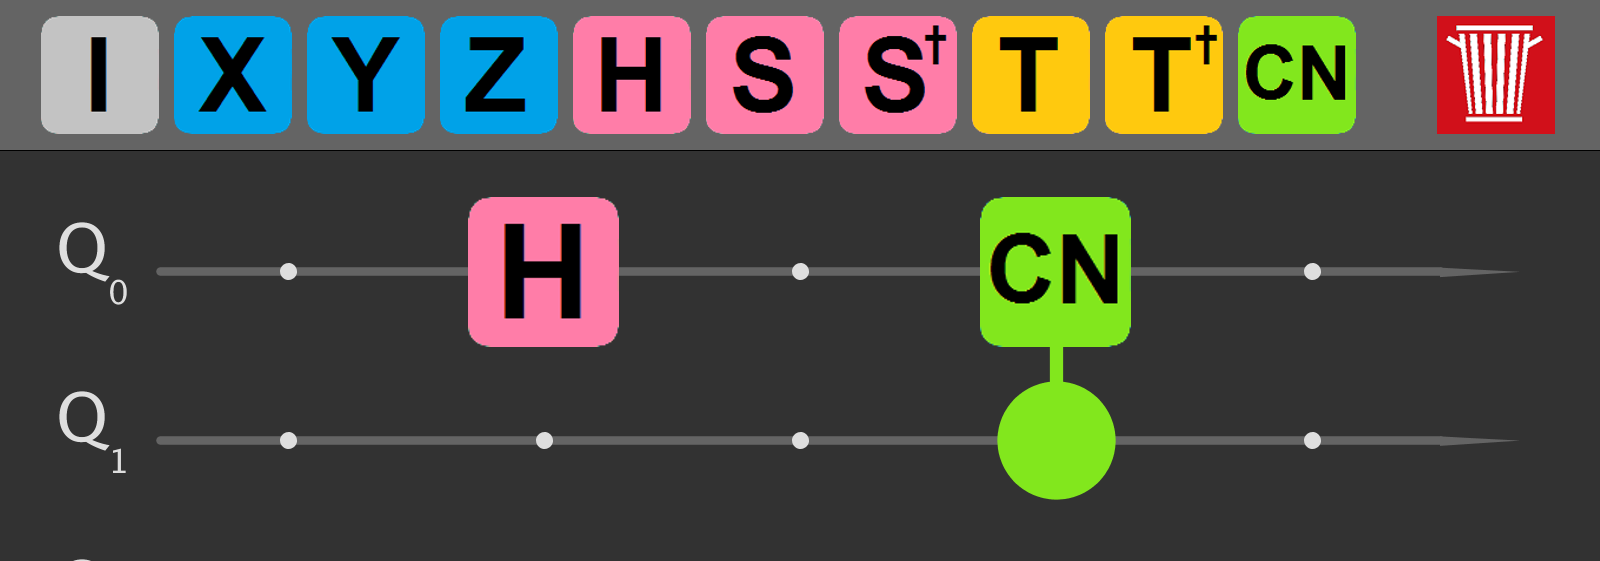
\includegraphics[width=\textwidth]{bell1.png}
	\caption{Erzeugung eines Bellzustandes}
	\end{figure}
\begin{align*}
	\ket{00}\cdot(\textbf{H}\otimes \textbf{I}) &= \frac{1}{\sqrt{2}}\cdot(\ket{00}+\ket{10})\\
	\frac{1}{\sqrt{2}}\cdot(\ket{10}+\ket{00})\cdot \textbf{CNOT} &= \frac{1}{\sqrt{2}}\cdot(\ket{00}+\ket{11})
\end{align*}
\end{frame}

\begin{frame}{Simulationsdemonstration}
\begin{figure}
    \subfigure{
    	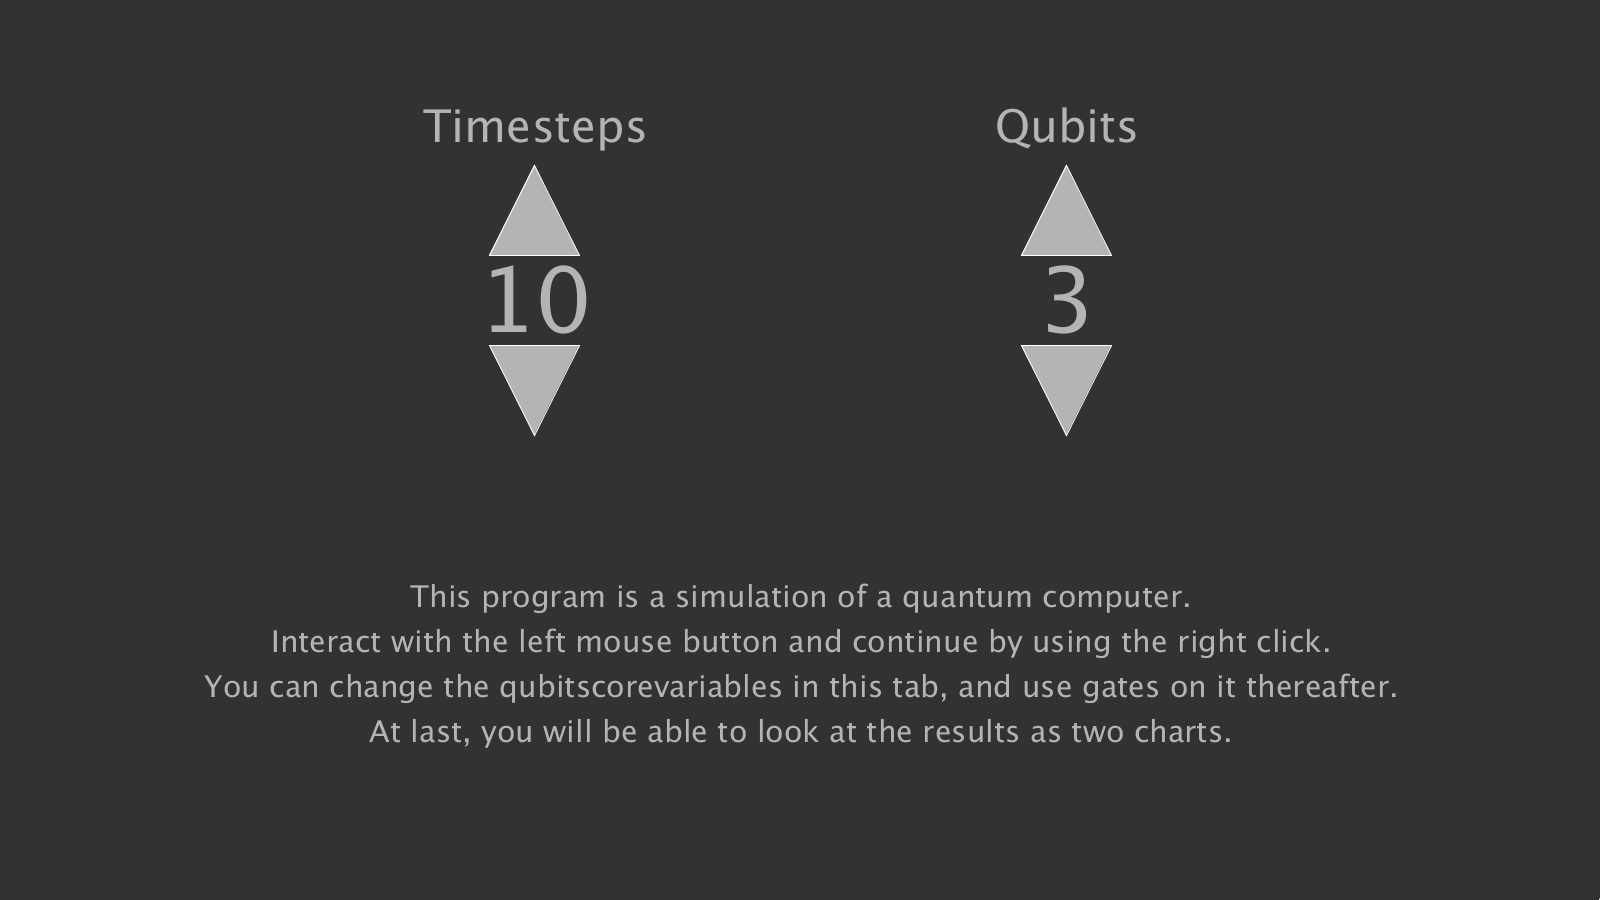
\includegraphics[width=0.47\textwidth]{e1.png}
    }
    \subfigure{
    	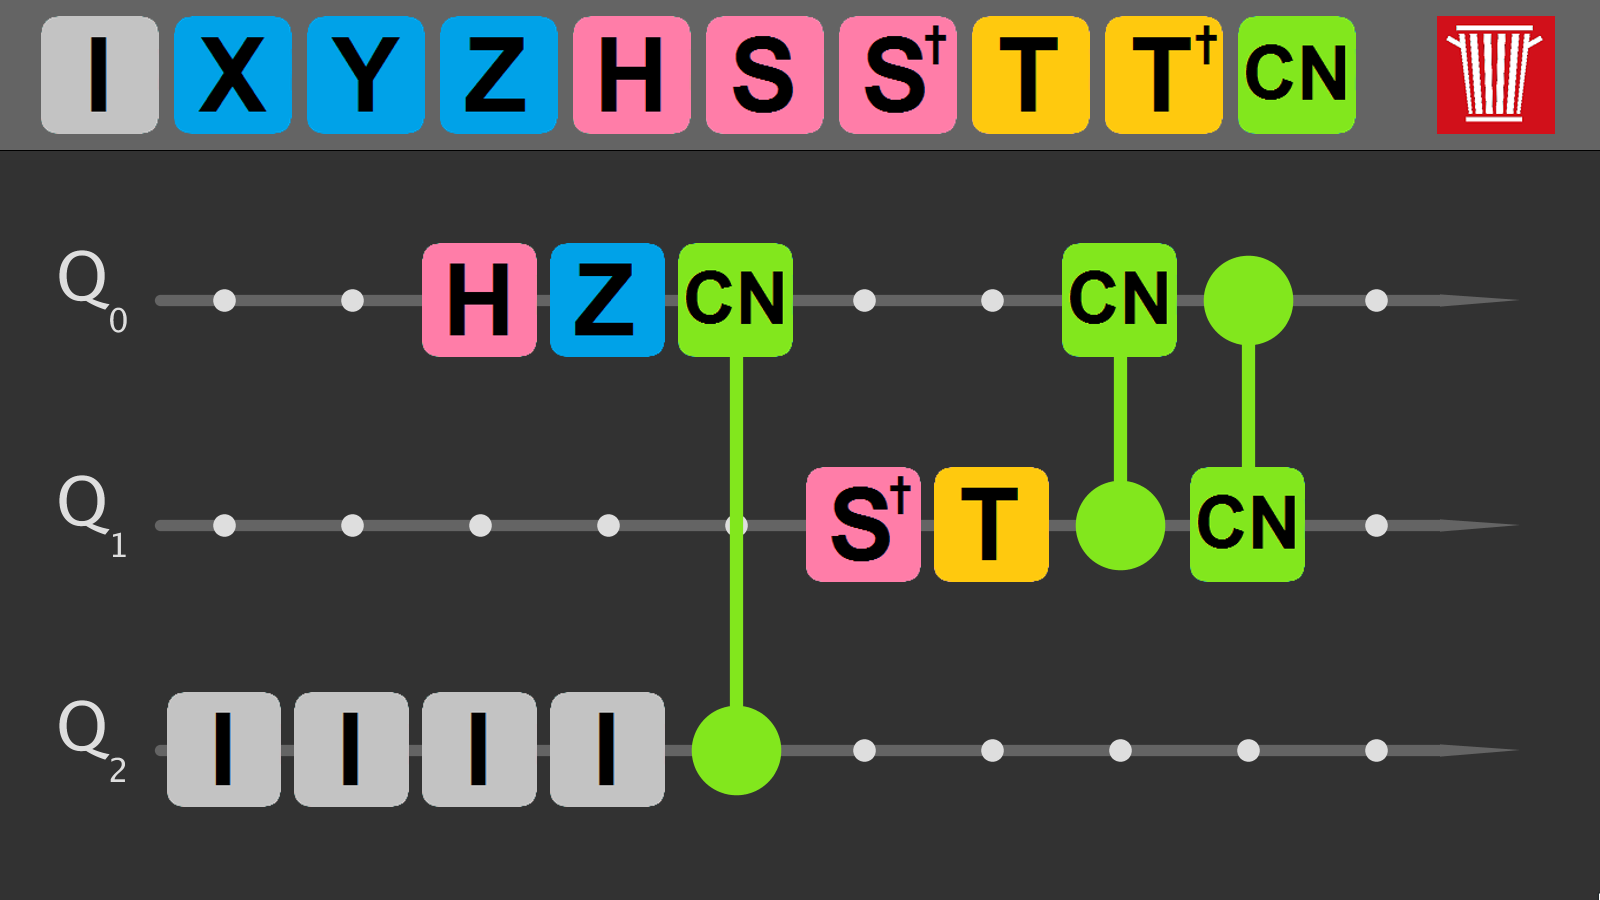
\includegraphics[width=0.47\textwidth]{e2.png}
    }
    \subfigure{
    	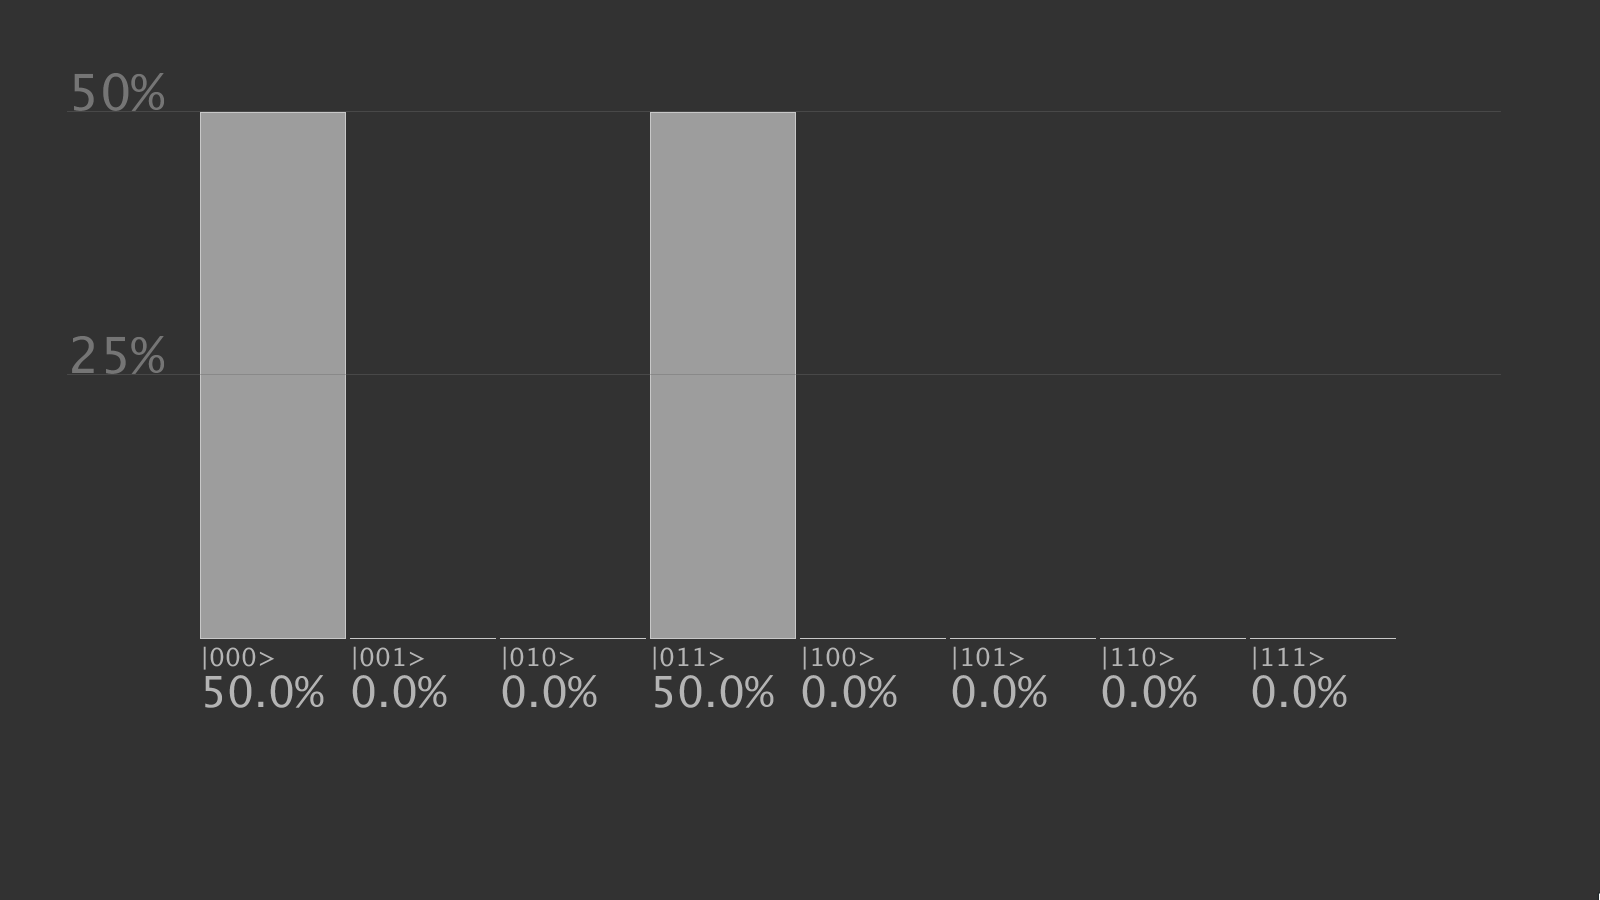
\includegraphics[width=0.47\textwidth]{e3.png}
    }
    \subfigure{
    	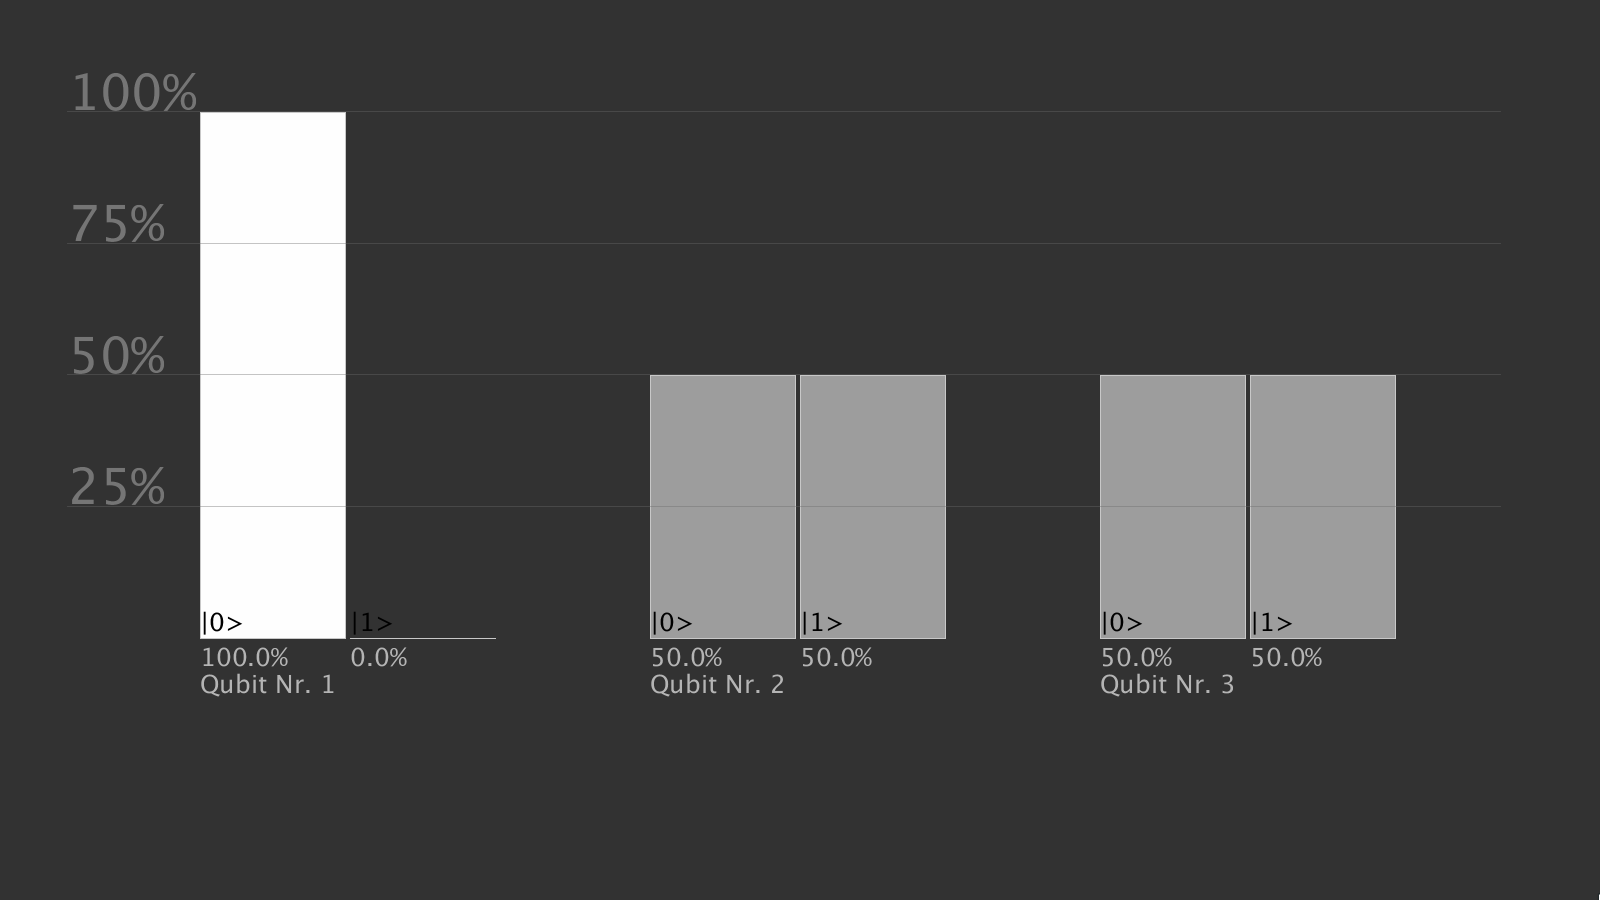
\includegraphics[width=0.47\textwidth]{e4.png}
    }
	\caption{Die Nutzungsoberflächen der Quantencomputersimulation}
	\end{figure}
\end{frame}

\section{Ausblick}
\begin{frame}{Aktueller Forschungsstand}
\begin{center}
\begin{figure}
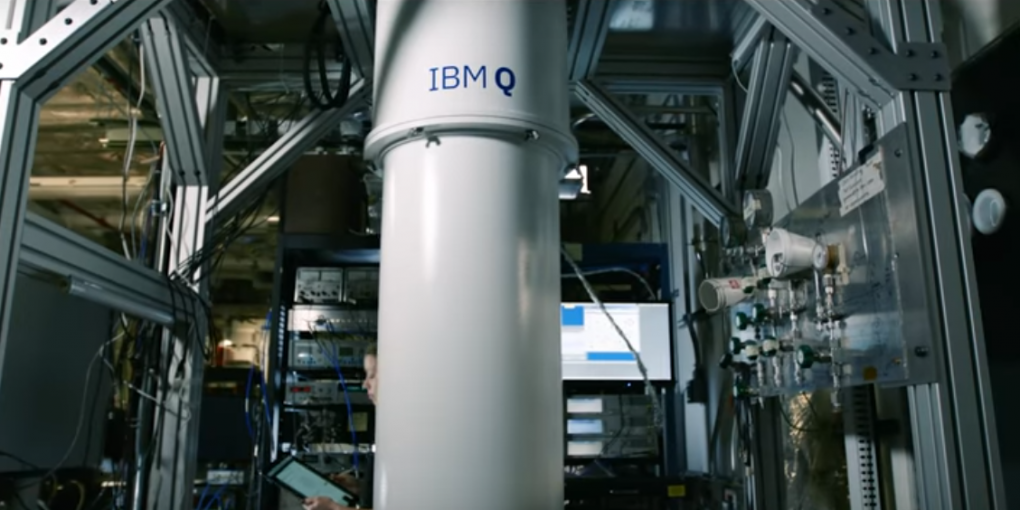
\includegraphics[width=0.47\textwidth]{ibmq.png}
\caption{IBM Q \newline \footnotesize{\url{https://i.ytimg.com/vi/2B680d-qvhI/maxresdefault.jpg}, 4.1.2018}}
\end{figure}
	\begin{itemize}
	\item Status der Grundlagenforschung
    \item Kein Quantencomputer außerhalb von Laboren
    \item Wenige Qubits
	\end{itemize}
\end{center}
\end{frame}

\begin{frame}{Ausblick}
\begin{center}
	\begin{itemize}
	\item Prognose schwierig
    \item große Investitionen und großes Engagement
    \item Beispiel: \textit{IBM Quantum Experience}
    \item Quantenrechner zukünftig in Großrechenzentren
	\end{itemize}
\end{center}
\end{frame}


\section{Quellen}

\begin{frame}{Quellen}
\begin{thebibliography}{9}
% DAS \FOOTNOTESIZE IMMER AN DEN ANFANG PACKEN
% bibitem([erstervornamebuschstabe][kapitelohnepunkte]-[footnotenumber])
\bibitem{p1}
\footnotesize Reich, Henry, Bell's Theorem: The Quantum Venn Diagram Paradox, Youtube, September 2017
\\\url{https://www.youtube.com/watch?v=zcqZHYo7ONs}, 30.12.2017
\bibitem{p2}
\footnotesize Greiter, Gebhard, Lokaler Realismus — was genau ist das?, Greiterweb, Dezember 2017
\\\url{http://greiterweb.de/spw/Lokaler-Realismus.htm}, 1.1.2018
\bibitem{p3}
\footnotesize Heigeartaigh, Colm, Qubits - Superposition and Entanglement, Redbrick, Mai 2003
\\\url{https://www.redbrick.dcu.ie/~hego/technicalmanual/node34.html},~1.1.2018

\end{thebibliography}
\end{frame}

\begin{frame}{Quellen}
\begin{thebibliography}{9}
% DAS \FOOTNOTESIZE IMMER AN DEN ANFANG PACKEN
% bibitem([erstervornamebuschstabe][kapitelohnepunkte]-[footnotenumber])

\bibitem{j1}
\footnotesize Houston-Edwards, Kelsey, The Mathematics of Quantum Computers, Youtube, Februar 2017
\\ \url{https://www.youtube.com/watch?v=IrbJYsep45E&index=2&list=WL&t=255s}, 4.1.2018
\bibitem{j2}
\footnotesize Christian Paul \& Till Zoppke, Shor's Algorithm - Faktorisierung großer Zahlen mit einem Quantencomputer, FU-Berlin, 2002, \\ \url{http://page.mi.fu-berlin.de/alt/vorlesungen/sem02/shors-algorithm.pdf}, 1.1.2018

\end{thebibliography}
\end{frame}

\frame{\titlepage}

\end{document}
